\chapter{Treiber}
\label{chap:Treiber}

\section{Treiber Architektur}
\subsection{Anforderungen}
Der Treiber ist dafür verantwortlich Pakete aus Windows zu dem Server zu senden. Dabei müssen 3 Probleme gelöst werden:
\begin{itemize}
    \item Sammeln von IP Paketen aus Windows
    \item Verteilen von IP Paketen an Programme
    \item Kommunikation zwischen Treiber und Server
\end{itemize}
Außerdem müssen gewisse Standards von Performance, Stabilität und Ressourcenintensität gehalten werden. Dabei haben wir versucht folgende Metriken einzuhalten:
\begin{itemize}
    \item Maximale prozentuale CPU Auslastung von 3 \%, bei einer 100 MB/s Übertragungsrate auf einem (Prozessor von Tests einsetzten)
    \item Maximaler Speicherverbrauch von 300 Mega Byte bei Verwendung von 2 übertragenen Netzwerkadaptern über eine Dauer von 30 Minuten.
    \item Wenn es zum Absturz des Treibers kommen sollte, darf das Betriebssystem nicht mit abstürzen.
    \item Der Treiber sollte weiter funktionieren, auch wenn während des Betriebs ein Netzwerkadapter ausfällt.
\end{itemize}
Zur Bedienungsfreundlichkeit wird eine CLI zur Verfügung gestellt mit welcher folgende Operationen ermöglicht werden:
\begin{itemize}
    \item Konfigurieren des Treibers über JSON, Key-Value Dateien oder über die Konsole
    \item Starten und Stoppen der Kommunikation des Treibers mit dem Server
    \item Stoppen und Starten des Treibers
    \item Ausgabe von derzeitigen Einstellungen
\end{itemize}
Die CLI soll über eine lokale TCP Verbindung mit dem Treiber kommunizieren damit sichergestellt werden kann das andere Komponenten leicht eingebunden werden können.
\newpage
\subsection{Sammeln von IP Paketen in Windows}
Damit Pakete an den Server versendet werden können, müssen wir dafür sorgen, dass Pakete die von verschiedenen Programmen in Windows verschickt werden durch unseren Treiber laufen. Um Pakete entgegennehmen zu können muss ein virtueller Netzwerkadapter erstellt werden. Dazu verwenden wir den Netzwerktreiber Wintun\footnote[1]{\url{https://www.wintun.net/}, 2021-01-16 23:19 MEZ}. Dieser kann performant Pakete empfangen und versenden.
\newline
\newline
Wintun kann jetzt zwar Pakete empfangen. Windows weiß aber noch nicht das es Pakete in den virtuellen Netzwerkadapter umleiten muss. Dafür muss eine statische IP Route im Windows internen IP Routing Table\footnote[2]{\url{https://docs.microsoft.com/en-us/windows-server/administration/windows-commands/route_ws2008}, 2021-01-16 23:30 MEZ} eingetragen werden.
\newline
\newline
Nach diesen 2 Schritten werden von Programmen gesendete Pakete, von Windows mithilfe  der Informationen im IP Routing Table, an den Wintun Adapter gesendet und dort durch unseren Treiber verarbeitet.
\begin{figure}[H]
    \centering
    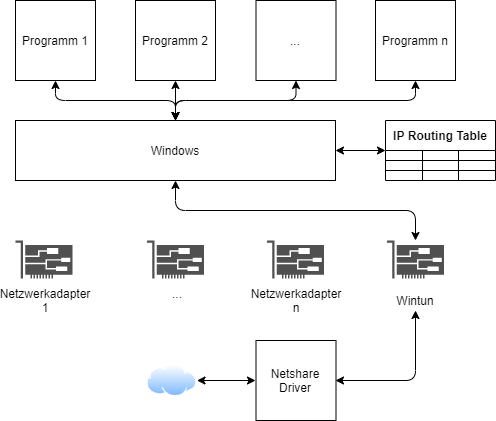
\includegraphics[width=0.8\textwidth]{diagramm_sammel_von_ip_paketen.png}
    \caption[Sammeln von IP Paketen]{Sammeln von IP Paketen \footnotemark[1]{Vgl. \ref{flasklogo}}} 
\end{figure}
\newpage
\subsection{Kommunikation zwischen Treiber und Server}
Der Treiber kann jetzt Pakete von Windows erhalten und muss diese jetzt an den Server schicken. Hierzu war die erste Entscheidung, die wir fällen haben mussten, auf welche Art wir die Pakete an den Server schicken. Dabei hatten wir zwei Möglichkeiten, die erste ist das wir Wintun zum Senden und Empfangen der Pakete vom Server benutzen oder wir erstellen einen Socket und lassen über diesen die Kommunikation mit dem Server laufen.
\newline
\newline
Wenn, wir Wintun verwenden würden hätten wir den Vorteil das wir keine weitere externe Bibliothek benutzen müssten und das wir eine höhere Performance hätten, weil wir Pakete von Schicht 3 versenden würde und uns dadurch eine Schicht beim Senden sparen würden.
\newline
\newline
Der Grund warum wir uns aber dazu entschieden haben Sockets zu nutzen ist der Programmieraufwand. Wir hätten zwar bei Wintun eine Performance Steigerung jedoch würde es auch Bedeuten, dass wir uns mit dem Aufbau der einzelnen IP Pakete beschäftigen müssen. Was alleine auch nicht allzu schlimm gewesen wäre, wenn wir uns nicht auch noch um die Firewalls kümmern müssten. Dadurch das Firewalls weiter oben im OSI Modell angelegt sind als unser TUN Gerät, müssen wir beim Empfangen von Paketen sichergehen, das die Firewall diese nicht wegwirft. Das heißt, wir müssten Windows mitteilen, dass wir einen gewissen Port benutzen und Pakete von einer gewissen IP-Adresse erwarten. Aus diesen beiden Gründen und durch unseren bestehenden Zeitdruck haben wir uns dazu entschieden eine Socket Bibliothek zu verwenden.
\newline
\newline
Für die Socket Bibliothek haben wir uns dann für die Windows Sockets 2 API entschieden, weil diese von Microsoft für das Performante verwenden von Sockets unter Windows entwickelt wurde. Außerdem haben wir den Vorteil das wir die Bibliothek nicht selber verwalten müssen, weil diese automatisch von Windows aktualisiert wird.
\subsection{Pakete auf Programme aufteilen}
Nachdem wir jetzt Pakete einsammeln können, diese dann an den Server schicken und empfangen können, müssen wir uns nur mehr darum kümmern, dass wir die Pakete aus unserem Treiber wieder an die Programme verteilen können, zu denen sie gehören.
\newline
\newline
Hierfür machen wir uns wieder Wintun zu nutzen, indem wir die Pakete, die wir bekommen haben, nehmen und einfach über unser Wintun Gerät senden. Windows erkennt dann, dass das Paket an sich selbst gerichtet ist und verarbeitet es als wäre es von einem normalen Adapter gekommen. Durch diese Art der Aufteilung lagern wir den meisten Programmieraufwand an Windows aus und können auch für eine hohe Performance garantieren.
\newpage
Fügt man nun alle 3 Überlegungen zusammen, kommt man auf Folgendes:
\begin{figure}[H]
    \centering
    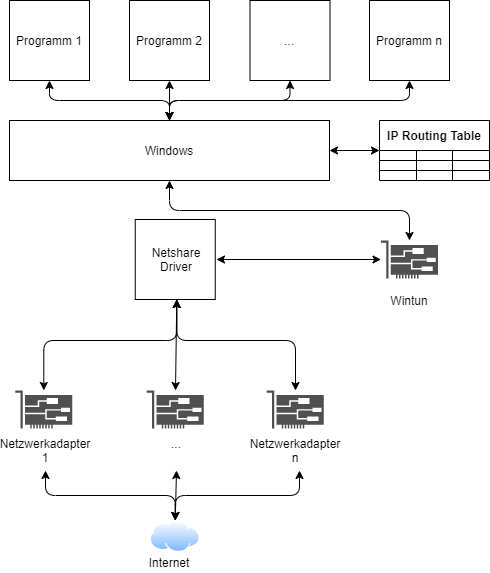
\includegraphics[width=0.8\textwidth]{kommunikation_mit_internet.png}
    \caption[Kommunikation mit Server]{Kommunikation mit Server \footnotemark[1]{Vgl. \ref{kommunikationMitInternet}}} 
\end{figure}